\documentclass{article}
\usepackage{tikz}
\usepackage{float} 
\usepackage{algorithm}
\usepackage{algpseudocode}

\title{Segment Trees in Algorithmic Problems}
\author{Piotr Szczepaniak}
\date{\today}

\begin{document}

\maketitle

\tableofcontents

\begin{abstract}
This document provides an overview of segment trees. In the first place
I will describe some algebraic topics which are necessary for better
understanding how and why segment trees works. This knowledge will be useful
for reading the rest of the paper where We will dive into different kinds of trees.
For each structure, I will explain how it work and how to apply it to problems.
Then, I will look at each structure's time complexity and space complexity.
\end{abstract}

\section{Foundations of Segment Trees}
A segment tree is a binary tree used for storing information about segments. 
To efficently retrieve or update informations about elements stored 
in segment tree we can perform various operations, the 
most common of which is the range query, range update or point update
(which is sipler case of range update). One of the examples of use can be maximum value of 
elements in given range or sum of elements in given range.

\begin{figure}[H]
    \centering
    
\begin{center}
    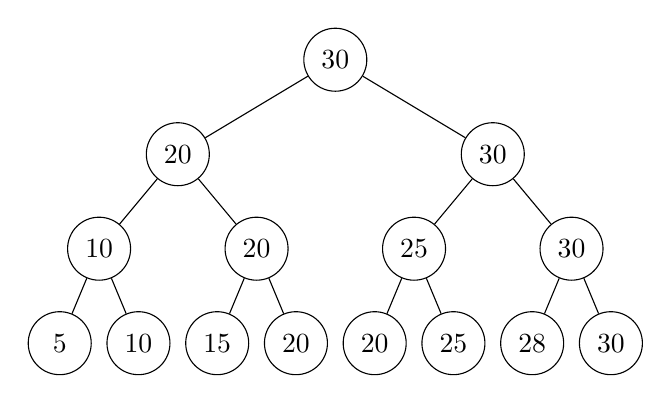
\begin{tikzpicture}[
      level distance=1.2cm,
      level 1/.style={sibling distance=4cm},
      level 2/.style={sibling distance=2cm},
      level 3/.style={sibling distance=1cm},
      every node/.style={draw,circle,minimum size=8mm,inner sep=1pt}
    ]
    
    % Root node with max value
    \node {30}
        child {node {20}
            child {node {10}
                child {node {5}}
                child {node {10}}
            }
            child {node {20}
                child {node {15}}
                child {node {20}}
            }
        }
        child {node {30}
            child {node {25}
                child {node {20}}
                child {node {25}}
            }
            child {node {30}
                child {node {28}}
                child {node {30}}
            }
        };
    
    \end{tikzpicture}
\end{center}
    \caption{Example of a segment tree with maximum value of elements in given range.}
    \label{fig:segment_tree_1}
\end{figure}

\subsection{Operation types}
To ilustrate use case of segment tree we will construct tree with max value on segment.
Let's say we are given an array \(A = [5, 10, 15, 20, 30, 25, 28, 20]\) of length \(n = 8\).
For now let's assume that the input array is of size \(n = 2^{k}\) where \(k\) is integer (for different
sizes of input we will fill input array with neutral elements (see section 2) to make it's length a power of 2).
The height of tree is \(h = \log_2{n}\). Let's define \(dep(i)\) as depth of node i in our tree.
We can see that \(dep(root) = 0\) and \(dep(leaf) = h\).
We want to be able to perform the following operations:
\begin{itemize}
    \item \textbf{Build structure} \\
    We will create a segment tree from an array.
    To build a segment tree, we need to create a binary tree where each node will store the maximum value of elements in its subtree. \\
    \begin{algorithm}
    \caption{Build Segment Tree for Maximum on Segment (Iterative)}
    \begin{algorithmic}
        \Procedure{BuildTree}{arr, seg}
            \For{$i = 0$ \textbf{to} $n - 1$} \Comment{Fill leaves of the segment tree}
                \State $seg[n + i] \gets A[i]$
            \EndFor
            \For{$i = n - 1$ \textbf{downto} $1$} \Comment{Calculates nodes from bottom to top}
                \State $seg[i] \gets \max(seg[2 \times i], seg[2 \times i + 1])$
            \EndFor
        \EndProcedure
    \end{algorithmic}
\end{algorithm}

    \item \textbf{Point update} \\
    Now let's update single value in the array and update the tree.
    We will change the value of \(A[1]\) from 10 to 35.
    To update the tree we need to change the value of the leaf node 
    and then update all the parent nodes up to the root.
    \begin{algorithm}
    \caption{Point Update on Segment Tree }
    \begin{algorithmic}
        \Procedure{update}{seg, index, value}
            \State $index \gets index + n$ \Comment{Shift index to leaf}
            \State $arr[index] \gets value$ \Comment{Update the value at the leaf}
            \While{$index > 1$} \Comment{Update the parent nodes}
                \State $index \gets \lfloor index / 2 \rfloor$
                \State $arr[index] \gets \max(arr[2 \times index], arr[2 \times index + 1])$
            \EndWhile
        \EndProcedure
    \end{algorithmic}
\end{algorithm}
    \begin{figure}[H]
        \centering
        
\begin{center}
    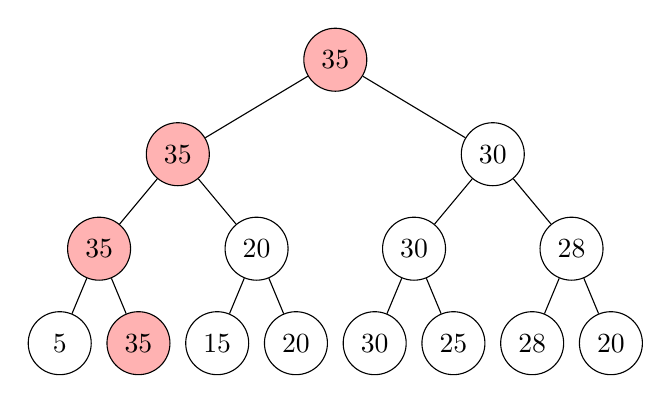
\begin{tikzpicture}[
      level distance=1.2cm,
      level 1/.style={sibling distance=4cm},
      level 2/.style={sibling distance=2cm},
      level 3/.style={sibling distance=1cm},
      every node/.style={draw,circle,minimum size=8mm,inner sep=1pt}
    ]
    
    % Root node with max value
    \node[fill=red!30] {35}
        child {node[fill=red!30] {35}
            child {node[fill=red!30] {35}
                child {node {5}}
                child {node[fill=red!30] {35}}
            }
            child {node {20}
                child {node {15}}
                child {node {20}}
            }
        }
        child {node {30}
            child {node {30}
                child {node {30}}
                child {node {25}}
            }
            child {node {28}
                child {node {28}}
                child {node {20}}
            }
        };
    
    \end{tikzpicture}
\end{center}

        \caption{Example of point update.}
        \label{fig:segment_tree_2}
    \end{figure}

    \item \textbf{Range query} \\
    Now let's say we want to find the maximum value in the range \(A[2:7]\).
    To do this we need to traverse the tree from the root to the leaves and 
    find nodes that are in the range. Then we will get max the values of these nodes to get the final result.
    To get the result for range \(A[2:7]\) we call \(RangeQuery(seg, 1, 1, 8, 2, 7)\).

    \begin{algorithm}
    \caption{Range Maximum Query on Segment Tree (Recursive, Close-Open Range)}
    \begin{algorithmic}[1]
        \Procedure{RangeQuery}{seg, index, l, r, a, b}
            \Comment{index: current node index in seg}
            \Comment{[l, r): segment represented by current node}
            \Comment{[a, b): query range}
            \If{$b \le l$ \textbf{or} $r \le a$}
                \State \Return $-\infty$ \Comment{No overlap}
            \ElsIf{$a \le l$ \textbf{and} $r \le b$}
                \State \Return $seg[index]$ \Comment{Total overlap}
            \Else
                \State $mid \gets \left\lfloor \frac{l + r}{2} \right\rfloor$
                \State $left \gets$ \Call{RangeQuery}{seg, $2 \cdot index$, $l$, $mid$, $a$, $b$}
                \State $right \gets$ \Call{RangeQuery}{seg, $2 \cdot index + 1$, $mid$, $r$, $a$, $b$}
                \State \Return $\max(left, right)$
            \EndIf
        \EndProcedure
    \end{algorithmic}
\end{algorithm}

    \begin{figure}[H]
        \centering
        
\begin{center}
    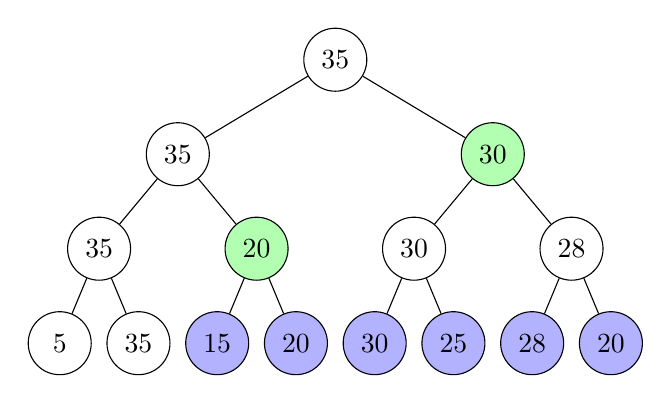
\begin{tikzpicture}[
      level distance=1.2cm,
      level 1/.style={sibling distance=4cm},
      level 2/.style={sibling distance=2cm},
      level 3/.style={sibling distance=1cm},
      every node/.style={draw,circle,minimum size=8mm,inner sep=1pt}
    ]
    
    % Root node with max value
    \node {35}
        child {node {35}
            child {node {35}
                child {node {5}}
                child {node {35}}
            }
            child {node[fill=green!30] {20}
                child {node[fill=blue!30]  {15}}
                child {node[fill=blue!30]  {20}}
            }
        }
        child {node[fill=green!30]  {30}
            child {node {30}
                child {node[fill=blue!30]  {30}}
                child {node[fill=blue!30]  {25}}
            }
            child {node  {28}
                child {node[fill=blue!30]  {28}}
                child {node[fill=blue!30] {20}}
            }
        };
    
    \end{tikzpicture}
\end{center}

        \caption{Example of range query. Blue leafs represents subarray \(A[2:7]\). Green nodes 
        represents nodes where ranges totally overlap and we can get max value. The result of the query is 30.}
        \label{fig:segment_tree_2}
    \end{figure}

\end{itemize}



\subsection{Monoids}
A monoid \( (S, e, \ast) \) is a set equipped with an associative binary operation \( S \times S \to S \) and
an identity element \(e\). 
\begin{itemize}
    \item \textbf{Associativity} \\
    For all \( a, b, c \in S \), \( (a \ast b) \ast c = a \ast (b \ast c) \).
    \item \textbf{Identity element} \\
    There exists an element \( e \in S \) such that for all \( a \in S \), \( a \ast e = e \ast a = a \).
\end{itemize}


\end{document}